% readme.tex -- a short example of how each Stata Journal insert should be
% organized.

\inserttype[st0001]{article}
\author{Reiner and Vilhuber}{%
  Lydia Reiner\\Independent researcher\\TX, USA\\lr397@cornell.edu
  \and
  Lars Vilhuber\\Cornell University\\Ithaca, NY, USA\\lars.vilhuber@cornell.edu
}
\title[{\tt packagesearch}]{Identifying packages used in Stata code}
\maketitle



\begin{abstract}
Many researchers work on personal machines, and have accumulated many installed packages over the years. Reproducibility of code requires that all packages used within an analysis be listed. While the robust solution is to install packages once, in a project-specific directory, most users appear to use their system-wide installations to store packages. When the time comes to create a reproducible package, this package helps such users to identify the packages actually used in their code, by parsing the Stata code and listing the most likely packages being used. We outline two use cases for this package. 

\keywords{\inserttag, packagesearch, reproducibility, replication package}
\end{abstract}

\section{Introduction}


\subsection{Background}

Community-provided packages, published through this Journal, the Boston Statistical Software Components (\texttt{SSC}) archive \citep{cox2010}, and individually hosted ``net installable'' websites, are one of the strengths of Stata. They can be conveniently installed through point-and-click interfaces and Stata commands, and are readily available to augment the capabilities of Stata. In \whmonth{} \whyear{}, the top 10 Stata packages on \texttt{SSC} had a total of \whhits{} downloads.

The inspiration for this package comes from research work under the AEA Data Editor, verifying countless Stata-based replication packages. Amongst replication packages submitted to the AEA journals, 73 percent use Stata at least in part, ahead of Matlab \citep[22 percent, see][]{VilhuberAEAPap.Proc.2020}.

Many fail to provide replication requirements, or said requirements are incomplete. This results in running Stata code without the proper packages installed, leading to a time-consuming process of code breaking, installing the necessary missing package, then restarting the process until all packages have been identified. With this project, we aim to identify the necessary Stata packages in provided .do files before code is run, saving time and frustration for authors and replicators alike.

More broadly, this could help mitigate small aspects of the replication crisis by allowing both authors and replicators identify packages used in code. It could be extra relevant in cases where provided code is unable to be run, such as when confidential data is used as an input. 


\subsection{Description}

The \texttt{packagesearch} command has four basic components:

1. Collects and cleans list of all packages hosted at SSC (using the \texttt{ssc whatshot} command. 

2. Parses each .do file in a specified directory (and subdirectories), then cleans and appends them. This step involves removing commented lines and collapsing the contents of each .do file into unique words.

3. Matches the parsed files against the list of existing SSC packages

4. Exports the results of the match. Results are ranked in terms of their popularity at SSC, with less popular packages having a higher probability of false positivity.

\subsection{Further Discussion}

The output of this command is a `candidatepackages` file which gives a list of potential SSC packages required by the code based on the results of the match. If code was run, the user can then cross-reference the contents of this `candidatepackages` file with the actual packages required by the code.

Currently, the process yields many more packages than are actually used by the code ("false positives") due to a variety of factors. This includes user-contributed packages that are built on top of an existing command (e.g- \texttt{bys}) , or packages with names that are commonly found in Stata code files but in other applications (e.g- \texttt{white, dash, cluster}). 

As such, for each candidate package in the output file we give the probability of said package being a false positive. This probability is inversely related to the package's rank at SSC (i.e, the package's popularity). For example, a more popular package such as \texttt{estout} will have a much lower probability of false positivity than lesser known (and therefore lesser utilized) packages.


\subsection{Limitations (Room for Improvement?)}

As described above, the \texttt{packagesearch} command only scans .do files for packages found at SSC. As such, it currently cannot handle packages from Stata Journal or those obtained via \texttt{net install}. 
We gladly accept any contributions \href{https://github.com/lydreiner/Statapackagesearch}{(Github repository linked here)} to the project that may help expand the reach of the command.

We are currently running this command on any Stata-based replication package submitted to the AEA Data Editor, and using the results (both genuine packages found by the match and information on false positives) to further fine tune the process. We hope that in the future this will allow us to further refine the command and its functionality.  


% discussion of the Stata Press LaTeX package for Stata output.

\section{User's guide to stata.sty}

\texttt{stata.sty} is a {\LaTeX} package containing macros and environments to
help authors produce documents containing {\stata} output and syntax
diagrams.

\subsection{Citing the Stata manuals}

The macros for generating references to the {\stata} manuals are
given in table~\ref{table:manref}.

\clearpage
\begin{table}[h!]
\caption{Stata manual references}
\label{table:manref}
\begin{center}
\begin{tabular}{ll}
\hline
\noalign{\smallskip}
Example & Result\\ 
\noalign{\smallskip}
\hline
\noalign{\smallskip}
\verb+\bayesref{bayes}+ & \bayesref{bayes}\\
\verb+\cmref{cmchoiceset}+ & \cmref{cmchoiceset} \\
\verb+\dref{Data types}+ & \dref{Data types}\\
\verb+\dsgeref{dsge}+ & \dsgeref{dsge} \\
\verb+\ermref{eregress}+ & \ermref{eregress} \\
\verb+\fnref{Statistical functions}+ & \fnref{Statistical functions}\\
\verb+\fmmref{fmm:~betareg}+ & \fmmref{fmm:~betareg}\\
\verb+\grefa{Graph Editor}+ & \grefa{Graph Editor}\\
\verb+\grefb{graph}+ & \grefb{graph}\\
\verb+\grefci{line\_options}+ & \grefci{line\_options}\\
\verb+\grefdi{connectstyle}+ & \grefdi{connectstyle}\\
\verb+\gsref{6~Using the Data Editor}+ & \gsref{6~Using the Data Editor} \\
\verb+\irtref{irt}+ & \irtref{irt} \\
\verb+\lassoref{Lasso intro}+ & \lassoref{Lasso intro}\\
\verb+\metaref{meta}+ & \metaref{meta} \\
\verb+\meref{me}+ & \meref{me}\\
\verb+\mreff{Intro}+ & \mreff{Intro}\\
\verb+\mrefa{Ado}+ & \mrefa{Ado}\\
\verb+\mrefb{Declarations}+ & \mrefb{Declarations}\\
\verb+\mrefc{mata clear}+ & \mrefc{mata clear}\\
\verb+\mrefd{Matrix}+ & \mrefd{Matrix}\\
\verb+\mrefe{st\_view($\,$)}+ & \mrefe{st\_view($\,$)}\\
\verb+\mrefg{Glossary}+ & \mrefg{Glossary}\\
\verb+\miref{mi impute}+ & \miref{mi impute}\\
\verb+\mvref{cluster}+ & \mvref{cluster}\\
\verb+\pref{syntax}+ & \pref{syntax}\\
\verb+\pssrefa{Intro}+ & \pssrefa{Intro}\\
\verb+\pssrefb{power}+ & \pssrefb{power}\\
\verb+\pssrefc{ciwidth}+ & \pssrefc{ciwidth} \\
\verb+\pssrefd{Unbalanced designs}+ & \pssrefd{Unbalanced designs}\\
\verb+\pssrefe{Glossary}+ & \pssrefe{Glossary} \\
\verb+\pssref{Subject and author index}+ & \pssref{Subject and author index} \\
\verb+\rptref{Dynamic documents intro}+ & \rptref{Dynamic documents intro}\\
\verb+\rref{regress}+ & \rref{regress}\\
\verb+\spref{Intro}+ & \spref{Intro}\\
\verb+\stref{streg}+ & \stref{streg}\\
\verb+\svyref{svy:~tabulate oneway}+ & \svyref{svy:~tabulate oneway}\\
\verb+\tsref{arima}+ & \tsref{arima}\\
\verb+\uref{1~Read this---it will help}+ & \uref{1~Read this---it will help}\\
\verb+\xtref{xtreg}+ & \xtref{xtreg}\\
\noalign{\smallskip}
\hline
\end{tabular}
\end{center}
\end{table}

\clearpage
\subsection{Stata syntax}

Here is an example syntax display:

\begin{stsyntax}
\dunderbar{reg}ress
    \depvar\
    \optindepvars\
    \optif\
    \optin\
    \optweight\
    \optional{,
    \underbar{nocons}tant
    \underbar{h}ascons
    tsscons
    vce({\it vcetype\/})
    \underbar{l}evel(\num)
    \underbar{b}eta
    \underbar{ef}orm(\ststring)
    \dunderbar{dep}name(\varname)
    {\it display\_options}
    \underbar{nohe}ader
    \underbar{notab}le
    plus
    \underbar{ms}e1
    \underbar{coefl}egend}
\end{stsyntax}

\noindent
This syntax is generated by

\begin{stverbatim}
\begin{verbatim}
\begin{stsyntax}
\dunderbar{reg}ress
    \depvar\
    \optindepvars\
    \optif\
    \optin\
    \optweight\
    \optional{,
    \underbar{nocons}tant
    \underbar{h}ascons
    tsscons
    vce({\it vcetype\/})
    \underbar{l}evel(\num)
    \underbar{b}eta
    \underbar{ef}orm(\ststring)
    \dunderbar{dep}name(\varname)
    {\it display\_options}
    \underbar{nohe}ader
    \underbar{notab}le
    plus
    \underbar{ms}e1
    \underbar{coefl}egend}
\end{stsyntax}
\end{verbatim}
\end{stverbatim}

\noindent
Each command should be formatted using a separate \texttt{stsyntax}
environment.  Table~\ref{table:syntax} contains an example of each syntax
macro provided in \texttt{stata.sty}. 

\clearpage
\begin{table}[h!]
\caption{\stata{} syntax elements}
\label{table:syntax}
\fontsize{10}{14}\selectfont
\begin{center}
\begin{tabular}{ll@{\hspace{.5in}}ll}
\noalign{\smallskip}
\hline
\noalign{\smallskip}
Macro & Result
&
Macro & Result
\\
\noalign{\smallskip}
\hline
\noalign{\smallskip}
\verb+\LB+ & \LB
&
\verb+\ifexp+ & \ifexp
\\
\noalign{\smallskip}
\verb+\RB+ & \RB
&
\verb+\optif+ & \optif
\\
\noalign{\smallskip}
\verb+\varname+ & \varname
&
\verb+\inrange+ & \inrange
\\
\noalign{\smallskip}
\verb+\optvarname+ & \optvarname
&
\verb+\optin+ & \optin
\\
\noalign{\smallskip}
\verb+\varlist+ & \varlist
&
\verb+\eqexp+ & \eqexp
\\
\noalign{\smallskip}
\verb+\optvarlist+ & \optvarlist
&
\verb+\opteqexp+ & \opteqexp
\\
\noalign{\smallskip}
\verb+\newvarname+ & \newvarname
&
\verb+\byvarlist+ & \byvarlist
\\
\noalign{\smallskip}
\verb+\optnewvarname+ & \optnewvarname
&
\verb+\optby+ & \optby
\\
\noalign{\smallskip}
\verb+\newvarlist+ & \newvarlist
&
\verb+\optional{text}+ & \optional{text}
\\
\noalign{\smallskip}
\verb+\optnewvarlist+ & \optnewvarlist
&
\verb+\optweight+ & \optweight
\\
\noalign{\smallskip}
\verb+\depvar+ & \depvar
&
\verb+\num+ & \num
\\
\noalign{\smallskip}
\verb+\optindepvars+ & \optindepvars
&
\verb+\ststring+ & \ststring
\\
\noalign{\smallskip}
\verb+\opttype+ & \opttype
\\
\noalign{\smallskip}
\hline
\end{tabular}
\end{center}
\end{table}

\verb+\underbar+ is a standard macro that generates underlines.  The
\verb+\dunderbar+ macro from \texttt{stata.sty} generates the underlines for
words with descenders. For example,

\begin{itemize}
\item
\verb+{\tt \underbar{reg}ress}+ generates {\tt \underbar{reg}ress}

\item
\verb+{\tt \dunderbar{reg}ress}+ generates {\tt \dunderbar{reg}ress}

\end{itemize}

The plain \TeX{} macros \verb+\it+, \verb+\sl+, and \verb+\tt+ are
also available. \verb+\it+ should be used to denote ``replaceable''
words, such as {\it varname}. \verb+\sl+ can be used for emphasis but
should not be overused. \verb+\tt+ should be used to denote words that
are to be typed, such as command names.

When describing the options of a new command, the \verb+\hangpara+ and
\verb+\morehang+ commands provide a means to reproduce a paragraph style
similar to that of the Stata reference manuals.  For example,

\hangpara
{\tt level(\num)} specifies the confidence level, as a percentage,
for confidence intervals.  The default is {\tt level(95)} or as set by {\tt
set level}; see \uref{20.8~Specifying the width of confidence intervals}.

\clearpage
\noindent
was generated by

\begin{stverbatim}
\begin{verbatim}
\hangpara
{\tt level(\num)} specifies the confidence level, as a percentage,
for confidence intervals.  The default is {\tt level(95)} or as set by {\tt
set level}; see \uref{20.8~Specifying the width of confidence intervals}.
\end{verbatim}
\end{stverbatim}


\subsection{Stata output}
\label{sec:output}

When submitting {\sl Stata Journal\/} articles that contain {\stata} output,
also submit a do-file and all relevant datasets that reproduce the output
(do not forget to set the random-number seed when doing simulations).  Results
should be reproducible. Begin examples by loading the data. Code should be
written to respect a linesize of 80 characters. The
following is an example of the \texttt{stlog} environment containing output
from simple linear regression analysis on two variables in {\tt auto.dta}:

\begin{stlog}
. sysuse auto
(1978 Automobile Data)
{\smallskip}
. regress mpg weight
{\smallskip}
      Source {\VBAR}       SS       df       MS              Number of obs =      74
\HLI{13}{\PLUS}\HLI{30}           F(  1,    72) =  134.62
       Model {\VBAR}   1591.9902     1   1591.9902           Prob > F      =  0.0000
    Residual {\VBAR}  851.469256    72  11.8259619           R-squared     =  0.6515
\HLI{13}{\PLUS}\HLI{30}           Adj R-squared =  0.6467
       Total {\VBAR}  2443.45946    73  33.4720474           Root MSE      =  3.4389
{\smallskip}
\HLI{13}{\TOPT}\HLI{64}
         mpg {\VBAR}      Coef.   Std. Err.      t    P>|t|     [95\% Conf. Interval]
\HLI{13}{\PLUS}\HLI{64}
      weight {\VBAR}  -.0060087   .0005179   -11.60   0.000    -.0070411   -.0049763
       _cons {\VBAR}   39.44028   1.614003    24.44   0.000     36.22283    42.65774
\HLI{13}{\BOTT}\HLI{64}
\nullskip
\end{stlog}

\noindent
The above listing was included using

\begin{stverbatim}
\begin{verbatim}
\begin{stlog}
. sysuse auto
(1978 Automobile Data)
{\smallskip}
. regress mpg weight
{\smallskip}
      Source {\VBAR}       SS       df       MS              Number of obs =      74
\HLI{13}{\PLUS}\HLI{30}           F(  1,    72) =  134.62
       Model {\VBAR}   1591.9902     1   1591.9902           Prob > F      =  0.0000
    Residual {\VBAR}  851.469256    72  11.8259619           R-squared     =  0.6515
\HLI{13}{\PLUS}\HLI{30}           Adj R-squared =  0.6467
       Total {\VBAR}  2443.45946    73  33.4720474           Root MSE      =  3.4389
{\smallskip}
\HLI{13}{\TOPT}\HLI{64}
         mpg {\VBAR}      Coef.   Std. Err.      t    P>|t|     [95\% Conf. Interval]
\HLI{13}{\PLUS}\HLI{64}
      weight {\VBAR}  -.0060087   .0005179   -11.60   0.000    -.0070411   -.0049763
       _cons {\VBAR}   39.44028   1.614003    24.44   0.000     36.22283    42.65774
\HLI{13}{\BOTT}\HLI{64}
\nullskip
\end{stlog}
\end{verbatim}
\end{stverbatim}

\noindent
where \texttt{output1.log.tex} is a Stata log file converted to include \TeX{}
macros by using the \stcmd{sjlog} command (more on \stcmd{sjlog} shortly).
\verb+\nullskip+ adjusts the spacing around the log file.

\clearpage
On occasion, it is convenient (maybe even necessary) to be able to omit some of
the output or let it spill onto the next page.  Here is a listing containing
the details of the following discussion:

\begin{stverbatim}
\begin{verbatim}
\begin{stlog}
. sysuse auto
(1978 Automobile Data)
{\smallskip}
. regress mpg weight
{\smallskip}
\oom
{\smallskip}
\clearpage
\end{stlog}
\end{verbatim}
\end{stverbatim}

The \verb+\oom+ macro creates
a short message indicating omitted output in the following example, and the
\verb+\clearpage+ macro inserts a page break.

\begin{stlog}
. sysuse auto
(1978 Automobile Data)
{\smallskip}
. regress mpg weight
{\smallskip}
\oom
{\smallskip}
\clearpage
\end{stlog}

The output in \texttt{output1.log.tex} was generated from the following
\texttt{output.do}:

\begin{stlog}
* output.do
set more off
capture log close
{\smallskip}
sjlog using output1, replace
sysuse auto
regress mpg weight
sjlog close, replace
{\smallskip}
sort weight
predict yhat
set scheme sj
scatter mpg yhat weight, c(. l) s(x i)
graph export output1.eps, replace
{\smallskip}
exit

\end{stlog}

\noindent
\texttt{output.do} generates a \stcmd{.smcl} file, \stcmd{.log} file,
and \stcmd{.log.tex} file using \stcmd{sjlog}.  The actual file used in the
above listing was generated by

\begin{stlog}
. sjlog type output.do
\end{stlog}

\texttt{sjlog.ado} is provided in the Stata package for \stcmd{sjlatex}.
\stcmd{sjlog} is a Stata command that helps generate log output to be included
in {\LaTeX} documents using the \texttt{stlog} environment.  If you have
installed the \stcmd{sjlatex} package, see the help file for \stcmd{sjlog} for
more details.  The lines that make up the table output from \stcmd{regress}
are generated from line-drawing macros defined in \texttt{stata.sty}; these
were macros written using some font metrics defined in \citet{texbook}.

By default, \texttt{stlog} sets an 8-point font for the log.  Use the
\texttt{auto} option to turn this behavior off, allowing you to use the
current font size, or change it by using\\ \verb+\fontsize{#}{#}\selectfont+.
The call to \texttt{stlog} with the \texttt{auto} option looks like
\verb+\begin[auto]{stlog}+.

Here is an example where we are using a 12-point font.

\vspace{-.2in}
{\fontsize{12}{13}\selectfont
\begin{stlog}[auto]
. sjlog type output.do
\end{stlog}
}

\subsection{About tables}

Tables should be created using the standard \LaTeX{} methods.  See
\citet{latexbook} for a discussion and examples. Tables should be included in
the main text rather than at the end of the document. Tables should be called
out in the text prior to appearance.

\clearpage
There are many user-written commands that produce \LaTeX{} output, including
tables.  Christopher F. Baum has written \stcmd{outtable}, a Stata command for
creating \LaTeX{} tables from Stata matrices.  Ben Jann's well-known
\stcmd{estout} command can also produce \LaTeX{} output.  To find other
user-written commands that produce \LaTeX{} output, try

\begin{stlog}
. net search latex
\end{stlog}

\subsubsection{Tables with notes}

Table~\ref{Table4} shows the order and format to use for notes to tables.

\begin{table}[h!]
\begin{threeparttable}
\centering
\caption{Industrial clusters}
\label{Table4}
\begin{tabularx}{\textwidth}{X  p{1.5cm}  p{1pt}  X  p{1.5cm}}
\hline
\multicolumn{2}{c}{China} & & \multicolumn{2}{c}{United States} \\
\cline{1-2} \cline{4-5}
Core of cluster & Size (in $\num$ of units) & & Core of cluster & Size (in $\num$ of units) \\
\cline{1-2} \cline{4-5}
Construction & 28$^{\rm a}$ & & Public administration and defense; compulsory social
security & 30$^{\rm b}$ \\
Food, beverages, and tobacco & 3 & & Food, beverages, and tobacco & 2 \\
Textiles and textile products & 2 & & Chemicals and chemical products & 1 \\
Chemicals and chemical products & 1 & & Basic metals and fabricated metal & 1 \\
Transport equipment & 1 & & Transport equipment & 1 \\
\hline
\multicolumn{2}{l}{$L_a=0.602$***} & & \multicolumn{2}{l}{$L_a=0.567$} \\
\multicolumn{2}{l}{$L_w=0.828$**} & & \multicolumn{2}{l}{$L_w=0.837$} \\
\multicolumn{2}{l}{$L_m=0.335$*} & & \multicolumn{2}{l}{$L_m=0.287$} \\
\multicolumn{2}{l}{$K^*=5$} & & \multicolumn{2}{l}{$K^*=5$} \\
\multicolumn{2}{l}{$K=35$} & & \multicolumn{2}{l}{$K=35$} \\
\hline
\end{tabularx}
\begin{tablenotes}
\footnotesize
\item \textsc{source:} Pew Research Center.
\item \textsc{note:} U.S.~industrial clusters based on
U.S.~input--output flows of goods expressed in millions of dollars between 35
{\smrm ISIC} industries from the {\smrm WIOD} data. The minimum number of
clusters \texttt{k()} was set equal to five. The algorithm returns $L_a$,
$L_w$, and $L_m$, which refer to the average of the internal relative
flows, the population-weighted average of the internal relative
flows, and the minimum of the internal relative flows,
respectively. $K^*$ and $K$ refer to the number of defined regional clusters
and the number of distinct starting units, respectively.
\item $^{\rm a}$ This note pertains only to row 1 column 2.
\item $^{\rm b}$ This note pertains only to row 1 column 4.
\item *** denotes $p<0.01$; ** denotes $p<0.05$; * denotes $p<0.1$.
\end{tablenotes}
\end{threeparttable}
\end{table}

Order of notes should be
\vspace{-.08in}
\begin{enumerate}
\item source notes
\item notes applying to the whole table
\item notes applying to specific parts of the table
\item notes on significance levels
\end{enumerate}

Special notes:

\vspace{-.08in}
\begin{itemize}
\item Use \verb+\centering+ because the {\tt center} environment adds
unnecessary vertical spacing.

\item Place the \verb+\begin{threeparttable}+ line above the caption.

\end{itemize}

Tables should be included in the main text rather than at the end of the
document. Tables should be called out in the text prior to appearance.

\subsection{Encapsulated PostScript (EPS)}

You can include figures by using either \verb+\includegraphics+ or
\verb+\epsfig+.

\begin{stverbatim}
\begin{verbatim}
\begin{figure}[h!]
\begin{center}
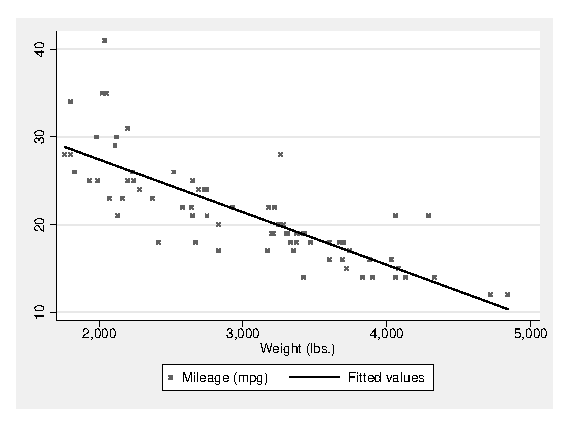
\includegraphics{eps/output1.eps}
\end{center}
\caption{Scatterplot with simple linear regression line}
\label{fig}
\end{figure}
\end{verbatim}
\end{stverbatim}

\begin{stverbatim}
\begin{verbatim}
\begin{figure}[h!]
\begin{center}
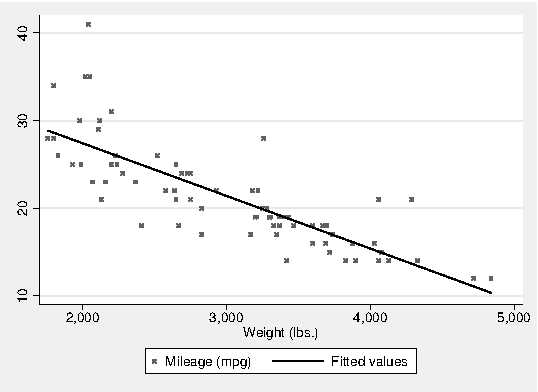
\epsfig{file=output1}
\end{center}
\caption{Scatterplot with simple linear regression line}
\label{fig}
\end{figure}
\end{verbatim}
\end{stverbatim}

Figure~\ref{fig} is included using \verb+\epsfig+ from the \texttt{epsfig}
package.  

\noindent
The graph was generated by running \texttt{output.do}, the
do-file given in section~\ref{sec:output}.  The \texttt{epsfig} package is
described in \citet*{latexcompanion}.

\clearpage

\begin{figure}[h!]
\begin{center}
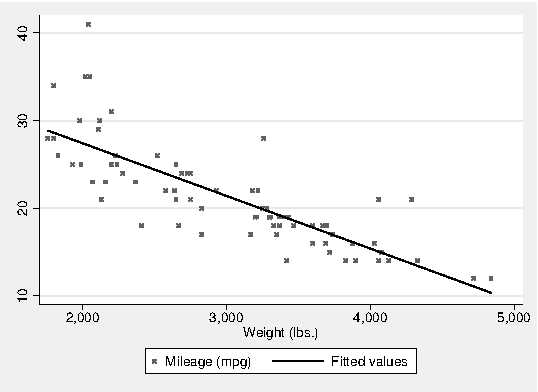
\epsfig{file=output1}
\end{center}
\caption{Scatterplot with simple linear regression line}
\label{fig}
\end{figure}

{\smrm EPS} is the preferred format for graphs and line art. Figures should be
included in the main text rather than at the end of the document and should be
called out in the text prior to appearance. If your article is written in
Word, you should submit your figures as separate {\smrm EPS} files. Rasterized-based
files of at least 300 dpi (dots per inch) are acceptable. Avoid using bitmaps
for figures and graphs, because even if images are outputted at 300 dpi,
bitmaps can increase the size of the resulting file for printing. (However,
bitmaps will be allowed for photographs, which are used in, for example, the
{\sl Stata Journal} Editors' prize announcement.) Images should be submitted in
black and white (grayscale). We recommend that graphs created in Stata use the
{\tt sj} scheme.

\subsection{Stored results}

The \texttt{stresults} environment provides a table to describe the stored
results of a Stata command.  It consists of four columns: the first and third
column are for Stata result identifiers (for example, \stcmd{r(N)},
\stcmd{e(cmd)}), and the second and fourth columns are for a brief description
of the respective identifier.
%
Each group of results is generated using the \verb+\stresultsgroup+ macro.
%
The following is an example containing a brief description of the results that
\stcmd{regress} stored to \stcmd{e()}:

\clearpage

\begin{stresults}
\stresultsgroup{Scalars} \\
\stcmd{e(N)} & number of observations
&
\stcmd{e(F)} & $\scriptstyle F$ statistic
\\
\stcmd{e(mss)} & model sum of squares
&
\stcmd{e(rmse)} & root mean squared error
\\
\stcmd{e(df\_m)} & model degrees of freedom
&
\stcmd{e(ll\_r)} & log likelihood
\\
\stcmd{e(rss)} & residual sum of squares
&
\stcmd{e(ll\_r0)} & log likelihood, constant-only\\
\stcmd{e(df\_r)} & residual degrees of freedom
&
& \quad model \\
\stcmd{e(r2)} & $\scriptstyle R$-squared
&
\stcmd{e(N\_clust)} & number of clusters
\\
\stresultsgroup{Macros} \\
\stcmd{e(cmd)} & \stcmd{regress}
&
\stcmd{e(wexp)} & weight expression
\\
\stcmd{e(depvar)} & name of dependent variable
&
\stcmd{e(clustvar)} & name of cluster variable
\\
\stcmd{e(model)} & \stcmd{ols} or \stcmd{iv}
&
\stcmd{e(vcetype)} & title used to label Std.~Err.
\\
\stcmd{e(wtype)} & weight type
&
\stcmd{e(predict)} & program used to implement
\\
&&&\quad \stcmd{predict}
\\
\stresultsgroup{Matrices} \\
\stcmd{e(b)} & coefficient vector
&
\stcmd{e(V)} & variance--covariance matrix of
\\
&&&\quad the estimators\\
\stresultsgroup{Functions} \\
\stcmd{e(sample)} & marks estimation sample
\\
\end{stresults}

Alternatively, you can use the \texttt{stresults2} environment to create
a two column table.   This format works better if your descriptions are long.

\subsection{Examples and notes}

The following are environments for examples and notes similar to those
given in the Stata reference manuals.  They are generated using the
\texttt{stexample} and \texttt{sttech} environments, respectively.


\begin{stexample}
This is the default alignment for a \stata{} example.
\end{stexample}

\setlength{\stexamplehskip}{0pt}
\begin{stexample}
For this example, \verb+\stexamplehskip+ was set to
\texttt{\the\stexamplehskip}
before beginning.  This sentence is supposed to spill
over to the next line, thus revealing that the first sentence was indented.

This sentence is supposed to show that new paragraphs are automatically
indented (provided that \verb+\parindent+ is nonzero).
\end{stexample}

\clearpage
\begin{sttech}
For this note, \verb+\sttechhskip+ was set to \texttt{\the\sttechhskip}
(the default) before beginning.  This sentence is supposed to spill over to
the next line, thus revealing that the first sentence was indented.

This sentence is supposed to show that new paragraphs are automatically
indented (provided that \verb+\parindent+ is nonzero).
\end{sttech}

\subsection{Special characters}

Table \ref{table:specialch} contains macros that generate some useful
characters in the typewriter (fixed width) font.  The exceptions are
\verb+\stcaret+ and \verb+\sttilde+, which use the currently specified font;
the strictly fixed-width versions are \verb+\caret+ and \verb+\tytilde+,
respectively.

\begin{table}[h!]
\caption{Special characters}
\label{table:specialch}
\begin{center}
\begin{tabular}{ll@{\hspace{.5in}}ll}
\hline
\noalign{\smallskip}
Macro & Result &
Macro & Result \\ 
\noalign{\smallskip}
\hline
\noalign{\smallskip}
\verb+\stbackslash+ & \stbackslash
 &
\verb+\sttilde+ & \sttilde
\\
\verb+\stforslash+ & \stforslash 
&
\verb+\tytilde+ & \tytilde
\\
\verb+\stcaret+ & \stcaret
&
\verb+\lbr+ & \lbr
\\
\verb+\caret+ & \caret
&
\verb+\rbr+ & \rbr
\\
\noalign{\smallskip}
\hline
\end{tabular}
\end{center}
\end{table}


\subsection{Equations and formulas}

In (\ref{eq:Exbar}), $\stbar{x}$ was generated using
\verb+\stbar{x}+.  Here \verb+\stbar+ is equivalent to the \TeX{} macro
\verb+\overline+.

\begin{equation}
E(\stbar{x}) = \mu
\label{eq:Exbar}
\end{equation}

In (\ref{eq:varbetahat}), $\sthat{\beta}$ was generated using
\verb+\sthat{\beta}+.  Here \verb+\sthat+ is equivalent to the \TeX{} macro
\verb+\widehat+.

\begin{equation}
V(\sthat{\beta}) = V\{(X'X)^{-1}X'y\} = (X'X)^{-1}X'V(y)X(X'X)^{-1}
\label{eq:varbetahat}
\end{equation}

\clearpage

Formulas should be defined and follow a concise style. Different
disciplines adhere to different notation styles; however, if the
notation cannot be clearly interpreted, you may be asked to make
changes. The bolding and font selection guidelines are the following:

\begin{itemize}
\item
	Matrices are capitalized and bolded; for instance, $\boldsymbol\Pi +
	\boldsymbol\Theta + \boldsymbol\Phi - \mathbf{B}$.

\item
	Vectors are lowercased and bolded; for instance, $\boldsymbol\pi +
	\boldsymbol\theta + \boldsymbol\phi - \mathbf{b}$.

\item
        Scalars are lowercased and nonbolded; for instance, $r_2 + c_1 - c_2$.
\end{itemize}


Sentence punctuation should not be used in formulas set off from the text.

Formulas in line with the text should use the solidus (/) instead of a
horizontal line for fractional terms.

Nesting of grouping is square brackets, curly braces, and then parentheses, or
[\{()\}].

Only those equations explicitly referred to in the text should be assigned an
equation number.

%\subsection{Other miscellaneous macros and environments}
%
%The following box was created by
%
%\begin{stverbatim}
%\begin{verbatim}
%\fbox{
%A special framed
%box that obeys lines and spaces.
%}
%\end{verbatim}
%\end{stverbatim}
%
%\fbox{
%A special framed
%box that obeys lines and spaces.
%}
%
%The following box was created by
%
%\begin{stverbatim}
%\begin{verbatim}
%\fbox{
%Test that the width of the
%box is \the\ttboxWd
%and is indented \the\ttboxIndent
%}
%\end{verbatim}
%\end{stverbatim}
%
%\fbox{
%Test that the width of the
%box is \the\ttboxWd
%and is indented \the\ttboxIndent
%}
%
\endinput





\bibliographystyle{sj}
\bibliography{statapackagesearch}

\begin{aboutauthors}
Lydia Reiner was an undergraduate at Cornell University studying economics when developing this package. She is now... (UPDATE).

Lars Vilhuber is an economist at Cornell University, and currently the Data Editor for the American Economic Association, responsible for verifying the computational reproducibility of manuscripts submitted to the AEA's various journals.

\textbf{Author Contributions}
LR came up with the idea, did the research, implemented and tested the code, and wrote the manuscript.

LV assisted with the code, tested the code, and wrote the manuscript.

\end{aboutauthors}

% Appendix describes how to compute the domain "econ"

\newpage
%\appendix
\begin{center}
	\large Appendix
\end{center}
\setcounter{section}{0}
\renewcommand{\thesection}{Appendix \arabic{section}}   

\section{Computing domain-specific frequencies}
\newcommand{\anaearep}{665}
\newcommand{\anaearepp}{546}
\newcommand{\asumado}{17471}
\newcommand{\asumdo}{13529}
\newcommand{\asumlines}{3722306}
\newcommand{\aadocount}{32}
\newcommand{\adocount}{25}
\newcommand{\adolines}{6817}


Instead of using the output of \texttt{ssc whatshot} to classify strings into likely package names, we have also allowed for the use of domain-specific frequencies. Such frequencies need to come from a large corpus of verified code. In this appendix, we describe how we computed these frequencies for the economics domain (invoked through option \texttt{domain(econ)}).

As part of the AEA Data Editors work, students download replication packages and attempt to run the code in combination with the available data. They do so in a (nearly) clean environment, by invoking the following commands at the start of the command execution:

\begin{stlog}
/* install any packages locally */
capture mkdir "$rootdir/ado"
sysdir set PERSONAL "$rootdir/ado/personal"
sysdir set PLUS     "$rootdir/ado/plus"
sysdir set SITE     "$rootdir/ado/site"
local ssc\_packages "pkg1 pkg2"
{\smallskip}
if !missing("`ssc\_packages'") {\lbr}
        foreach pkg in `ssc\_packages' {\lbr}
                capture which `pkg'
                if _rc == 111 {\lbr}                 
                        dis "Installing `pkg'"
                        ssc install `pkg', replace
                {\rbr}
                which `pkg'
        {\rbr}
{\rbr}
\nullskip
\end{stlog}

These commands should ensure that all necessary packages must be installed into a project specific directory. In rare cases, replication packages may already include \texttt{ado} files, which should then be used. Once installed, the \texttt{ado} \textit{directory} should also be committed to the git repository tracking the reproducibility check.\footnote{Compliance with these instructions is not perfect.} The resulting updated (private) repository thus contains authors' Stata code, and the replicator's installed \texttt{ado} files. 

We thus obtained from our internal records the last known state of \anaearep{} repositories as of July 2021. Of these, \anaearepp{} contained at least one Stata do-file. The average replication package had \adocount{} do-files, and after verification had \aadocount{} ado-files. For each replication package, we ran (an earlier version of) the \texttt{packagesearch} command, and matched against the list of ado-files found. We counted as a \texttt{hit} a package that was confirmed to have the package installed, and counted the hits. We then ranked the list by hits. The resulting list is naturally somewhat different than the \texttt{whatshot} list, and in particular is pruned of spurious package names. Table~\ref{tab:econ} displays the top ten by the \texttt{domain(econ)} ranking, Table~\ref{tab:whatshot} displays the top ten packages per \texttt{whatshot} and their equivalent \texttt{domain(econ)} ranking.

\begin{table}[ht!]
		\centering
		\caption{Top ten \texttt{econ} packages.
		\label{tab:econ}}
	\begin{threeparttable}
		
\begin{tabular}{lrr}\toprule
Packagename&\texttt{econ}&\texttt{whatshot}\\\midrule
estout&1&2\\
reghdfe&2&5\\
outreg2&3&1\\
coefplot&4&13\\
ftools&5&6\\
ivreg2&6&8\\
ranktest&7&16\\
binscatter&8&24\\
spmap&9&25\\
unique&10&20\\
\bottomrule\end{tabular}


		\begin{tablenotes}
			\item \footnotesize Generated on 2022-01-30.
		\end{tablenotes}
	\end{threeparttable}
\end{table}

\begin{table}[ht!]
		\centering
		\caption{Top ten \texttt{whatshot} packages.}
		\label{tab:whatshot}
	\begin{threeparttable}
		
	\begin{tabular}{lrr}\toprule
Packagename&\texttt{econ}&\texttt{whatshot}\\\midrule
outreg2&3&1\\
estout&1&2\\
asdoc&&3\\
winsor2&51&4\\
reghdfe&2&5\\
ftools&5&6\\
logout&119&7\\
ivreg2&6&8\\
ivreg29&&9\\
ivreg210&&10\\
\bottomrule\end{tabular}
	
		
		\begin{tablenotes}
			\item \footnotesize Generated on 2022-01-30.
		\end{tablenotes}
	\end{threeparttable}
\end{table}

